\documentclass[letter, 10pt]{article}

%Multicolumna
\usepackage{multirow}

%Pseudo codigo
\usepackage{algpseudocode}

%Cambiado por problemas con tildes
\usepackage[utf8]{inputenc}
\usepackage[spanish]{babel}
\usepackage{amsfonts}
\usepackage{amsmath}
\usepackage{float}


%Cambiado por problemas con tikz
\usepackage{ifpdf}
\ifpdf
    \usepackage{graphicx}  %If run with `pdflatex`
\else
    \usepackage[dvips]{graphicx} %If run with `latex`
\fi


\usepackage{url}
\usepackage[top=3cm,bottom=3cm,left=3.5cm,right=3.5cm,footskip=1.5cm,headheight=1.5cm,headsep=.5cm,textheight=3cm]{geometry}


\usepackage{verbatim}
\usepackage{subcaption}


\usepackage{tikz}
\usetikzlibrary{babel,arrows}

\begin{document}
\title{Proyecto 1 \\ Multigrid}
\author{[Camilo Valenzuela Carrasco]}
\date{\today}
\maketitle


\section{Introducción}

En el ámbito de la ciencia aplicada es múy común modelar procesos físicos utilizando ecuaciones matemáticas que capturan el comportamiento de dicho proceso.

Un caso particual de estos modelos matemáticos son las ecuaciones diferenciales parciales (EDP) donde se busca una función matemática que cumpla dicha ecuación. En algunas ocasiones se puede encontrar la solución que cumple la ecuación de forma algebráica, pero existen EDP que no se pueden resolver de forma analítica por lo que se desarrollaron métodos para poder llegar a una solución aproximada de forma numérica.

La finalidad de este trabajo es analizar y comparar tres algoritmos iterativos que buscan resolver Ecuaciones Diferenciales Parciales de forma numérica. Se comenzará realizando una pequeña descripción de cada algoritmo, luego se describirá el problema que se intenta resolver, la implementación realizada y los resultados obtenidos, para finalizar con las conclusiones realizadas a partir de los resultados obtenidos.


\section{Discretización}

Una Ecuación Diferencial Parcial (EDP) generalmente está definida en un dominio continuo, dependiendo del tipo de EDP este dominio puede estar acotado en un intervalo $[a,b]$ o no acotado.

Las EDP con dominio acotado se denominan Boundary Value Problem (BVP) o Problema de Valor de Frontera, este dominio acotado se puede dividir en N puntos donde la distancia entre los puntos es:

\begin{equation}
     |x_n - x_{n+1}| =   h = \frac{b-a}{N}
\end{equation}

Además en este tipo de ecuaciones se puede discretizar las derivadas parciales de la ecuación utilizando una técnica llama \textit{diferencias finitas} que se basa en una expansión de taylor para poder aproximar dichas derivadas. Un ejemplo de una derivada parcial utilizando discretización de segundo orden queda de la forma

\begin{align}
     \frac{\delta^2 u}{\delta x^2} = \frac{u_{i-1} - 2 u_i + u_{i+1}}{h^2} \\
     \text{Con: }  u(a) = c_1, u(b) = c_2
\end{align}

Dada un BVP de la forma
\begin{equation}
  \frac{\delta^2 u}{\delta x^2} = f(x)   
\end{equation}

Se puede discretizar de la forma

\begin{equation}
  U_{i-1} - 2 U_i + U_{i+1} = h^2 f(x_i), \text{ con } i=1\dots N
\end{equation}

Que de forma matricial queda
\begin{equation}
    \begin{bmatrix}
        -2      & 1 & 0 & 0 \dots & 0 \\
        1       & -2 & 1 & 0 \dots & 0\\
        \ddots & \ddots & \ddots & 1 &-2
      
    \end{bmatrix}
    \cdot
    \begin{bmatrix}
       u_1 \\
       u_2 \\
       \vdots \\
       u_N
    \end{bmatrix}
    =
    h^2
    \begin{bmatrix}
    f(x_1) - c_1 \\
    f(x_2) \\
    \vdots \\
    f(x_N) - c_2
    \end{bmatrix}  
\end{equation}

Y se obtiene un sistema de ecuaciones lineales de la forma
\begin{equation}
    Au = f
\end{equation}

\section{Gauss Seidel}
El método de Gauss Seidel \cite{briggs2000multigrid} es un algoritmo iterativo que se utiliza para resolver sistema de ecuaciones lineales de la forma $Au = f$. La solución que entrega este algoritmo depende de un initial guess que se le entrega en la primera iteración, si el sistema cuenta con varias soluciones el método va a tender a encontrar la más cercana a ese initial guess.

Una propiedad importante de este algoritmo es que si la matriz es diagonal dominante ($a_{ii} >  \sum_{j\neq i} a_{ji}$), este método asegura convergencia.

El algoritmo puede ser descrito de la siguiente forma:
\begin{enumerate}
    \item Sea $v_0$ un initial guess, $v_n$ la solución aproximada en la iteración $n$,  $A$ una matriz cuadrada que se descompone de la forma $A = L + D + U$, Donde $L$ es una matriz triangular inferior, $D$ es una matriz diagonal y $U$ una matriz triangular superior, además la diagonal de D y U es igual a 0.
    \item El sistema $Av = f$ puede ser escrito de la forma
    \begin{align}
        (L + D + U)v &= f \\
        (L+D) v + Uv &= f   \\
        (L+D)v &= f - Uv \\
        v_{n+1} = (L+D)^{-1} &(f - Uv_{n})
    \end{align}
    
\end{enumerate}

A grandes rasgos este algoritmo comienza con un Initial Guess y en cada iteración va ajustando esta solución hasta llegar a un máximo de iteraciones o una toleracia mínima.

En el caso de buscar una tolerancia mínima se puede utilizar el residuo $||r^n||_2 = ||Av^n - f||_2$ que nos entrega una aprixmación del error $||e||_2 = ||u-v||_2$ donde $u$ es la solución exacta y $v$ es la aproximada. 

\section{V-cycle Scheme}

V-Cycle Scheme \cite{briggs2000multigrid} es un algoritmo que utiliza como base la relajación Gauss Seidel, pero en cada iteración de V-Cycle trata de corregir el error resolviendo problemas más pequeños y así buscando una convergencia más rápida.

Este algoritmo puede ser definido de forma recursiva, dado $\nu_1$ y $\nu_2$, un initial guess $v_0$ y una discretización del dominio en $N$ nodos con $h = \frac{|b-a|}{N}$ 
\begin{enumerate}
    \item Sea $v^h \rightarrow v-cycle^h(v^h,f^h)$
    \item Se realizan $\nu_1$ iteraciones o relajaciones Gauss Seidel a nuestra solución actual $v^h$.
    \item Se calcula
        \begin{equation}
            r^h = f^h - A^h v^h 
        \end{equation}
    \item Se restringe el residuo para llevarlo a una malla más gruesa
        \begin{equation}
            r^{2h} = I_h^{2h} r^{h} 
        \end{equation}
        Esto deja $r^{2h}$ con $\frac{N}{2^d}$ nodos, con $d$ la dimensión del dominio.
    \item Se realiza la llamada recursiva $e^{2h} \rightarrow v-cycle^{2h}(0,r^{2h})$
    \item Luego se interpola el error, volviendolo a una malla más fina
        \begin{equation}
            e^{h} = I_{2h}^{h} e^{2h} 
        \end{equation}
    \item Se corrige la solución actual $x^h = x^h + e^h$
    \item Finalmente se realizan $\nu_2$ relajaciones Gauss Seidel.
\end{enumerate}

\begin{figure}
    \centering
    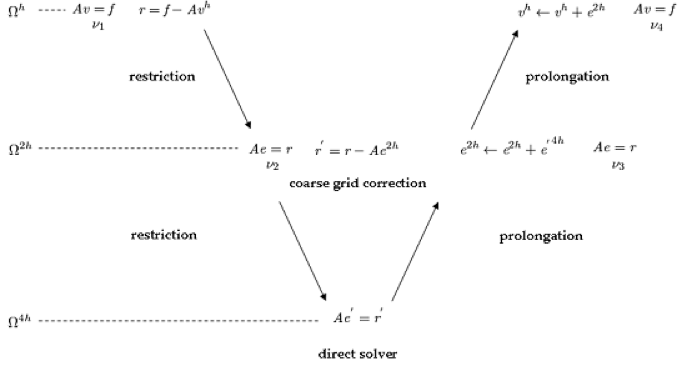
\includegraphics[scale=0.4]{vcycle.png}
    \caption{V-Cycle Scheme}
    \label{fig:vcyle}
\end{figure}
Al igual que en el método Gauss Seidel, V-Cycle se puede detener luego de cierta cantidad de iteraciones o con un umbral de la norma del residuo.


\section{Full Multigrid}

El algoritmo Full Multigrid (FMG) utiliza una idea parecida a V-cycle, a diferencia del algoritmo anterior, FMG trata de resolver siempre el mismo problema pero a distintas escalas comenzando por la escala
más gruesa y luego utilizando la solución obtenida como initial guess en la malla más gruesa así buscando una convergencia mucho más rápida.

Al igual que V-cycle este algoritmo se puede describir de forma recursiva, sean $\nu_0, \nu_1, \nu_2 \in \mathcal{N}$ FMG se define de la siguiente forma

\begin{enumerate}
    \item Sea $v^h \rightarrow FMG^h(f^h)$
    
    \item Si estamos en la malla más gruesa, $v^h \rightarrow 0$ se pasa directamente al paso 4.
    
    Si no 
    \begin{align}
         f^{2h} \rightarrow I_{h}^{2h} f^h\\
         v^{2h} \rightarrow FMG^{2h}(f^{2h})\\
    \end{align}
    \item Corregir $v^h \rightarrow I_{2h}^h{v^{2h}}$
    \item Se realiza $v^{h} \rightarrow v-cycle^h(v^{h},f^{h})$ $\nu_0$ veces, con los parámetros $\nu_1,\nu_2$ para $v-cycle^{h}$
\end{enumerate}

A diferencia de los algoritmos anteriores FMG es sólo una iteración, por lo que se necesita probar distintos parámetros de $\nu_0,\nu_1,\nu_2$ para encontrar la mejor combinación de ellos que entreguen el menor residuo.


Como Full Multigrid es un esquema como V-Cycle existen otros algoritmos parecidos, se implementó el FMG propuesto por  \cite{ye2001nonlinear}  que se detalla en la figura \ref{fig:FMG}.

\begin{figure}
    \centering
    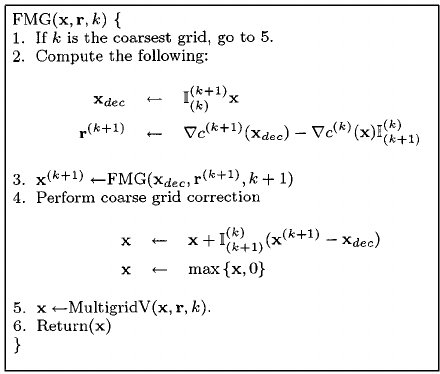
\includegraphics[scale=0.5]{FMG.png}
    \caption{Full Multigrid Residuo.}
    \label{fig:FMG}
\end{figure}


A diferencia del primer esquema FMG, en este caso se utiliza el residuo y la solución actual se va actualizando según el residuo de las mallas más gruesas (muy parecido a un esquema v-cycle), en este caso cuando se cambia de malla se resuelve un problema $Ae = r$, no como en el esquema normal de FMG que se resuelve siempre $Av=f$ en cada malla.


\section{Problema a resolver}

Se tiene la siguiente ecuación de poisson

\begin{align}
    \frac{\delta^2 u}{\delta x^2} + \frac{\delta^2 u}{\delta y^2} &= -2 \left[(1-6x^2) y^2 (1-y^2) + (1-6y^2) x^2 (1-x^2)\right] = f(x,y)  \\
     u = 0\text{ en }&x=0,x=1,y=0,y=1 \\
      0 \leq x&,y \leq 1
\end{align}

Se necesita encontrar una solución numérica para dicha ecuación utilizando los métodos previamente detallados.

\subsection{Discretización}
Para poder resolver la ecuación de forma numérica se realizó una discretizacion de segundo orden de la forma

\begin{equation}
     u_{xx} = \frac{ u_{i-1,j} - 2  u_{i,j} + u_{i+1,j} }{h^2}  , u_{yy} = \frac{ u_{i,j-1} - 2 u_{i,j} + u_{i,j+1} }{h^2}
\end{equation}

Donde $h = \frac{1}{N-1}$ y $N$ es la cantidad de nodos de la grilla.

Luego de reemplazar la ecuación nos queda de la forma:
\begin{equation}
    \frac{ u_{i-1,j} + u_{i,j-1} - 4 u_{i,j} + u_{i+1,j} + u_{i,j+1} }{h^2} = f_{i,j} 
\end{equation}


\section{Implementación}
    Para la implementación de los algoritmos se utilizó \textbf{Python} con el paquete \textbf{numba} para optimizar el código computacionalmente exigente.
    
    El algoritmo de \textbf{Gauss Seidel} se implementó utilizando la discretización previamente descrita agregando el índice $n$ de la iteración actual y $n+1$ de la iteración siguiente, por lo que la ecuación nos queda de la forma
    
    \begin{equation}
     u_{i,j}^{n+1} = \frac{- h^2f_{i,j}+u_{i-1,j}^{n+1} + u_{i,j-1}^{n+1}+ u_{i+1,j}^{n} + u_{i,j+1}^{n} }{4} 
    \end{equation}
    
    Suponiendo que recorremos la solución de arriba hacia abajo, de izquierda a derecha los valores de $u_{i-1,j}^{n+1} , u_{i,j-1}^{n+1}$ ya han sido calculados anteriormente, por lo que no necesitamos realizar operaciones más costosas para obtenerlos.

    Para el caso de \textbf{V-Cycle} y \textbf{Full Multigrid} se implementaron las funciones de restricción \textit{Injection} y \textit{Full Weight} con 8 vecinos (Ver figura \ref{fig:fw}), una función de interpolación que ocupa los 8 vecinos a un punto en la malla fina.
    
    \begin{figure}
        \centering
        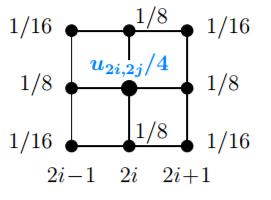
\includegraphics[scale=0.5]{fw.jpg}
        \caption{Full Weighted Restriction 8 Vecinos}
        \label{fig:fw}
    \end{figure}
    
\section{Experimentos}
Para comparar el comportamiento de estos algoritmos se realizaron dos experimentos
\begin{enumerate}
    \item Ver la cantidad de iteraciones, relajaciones Gauss Seidel equivalentes, error y tiempo de los tres algoritmos variando la cantidad de nodos de la discretización del dominio, además se probaron ambas restricciones para ver si existia un cambio en el comportamiento del algoritmo.
    \item Variar los parámetros $\nu_0,\nu_1,\nu_2$ dejando fija la cantidad de nodos para ver el impacto de estos parámetros.
\end{enumerate}

\section{Resultados y Conclusiones }

\subsection{Experimento 1}
Lo que se busca en este experimento es ver qué tan eficaces son los 3 algoritmos descritos anteriormente. En este experimento se corrieron los distintos algoritmos con $n= 65,129,257$.

Como era de esperarse la cantidad de iteraciones de cada algoritmo aumenta con la cantidad de nodos, en el caso de Gauss Seidel sólo esta cantidad crece exponencialmente a medida que aumenta la cantidad de nodos, para V-Cycle y FMG se ve que la cantidad de iteraciones aumenta casi de forma lineal utilizando Full Weighted y Injection como funciones de restricción como se puede ver en las figuras \ref{fig:fw_iters} y \ref{fig:iters}. 


\begin{figure}[H]
    \centering
    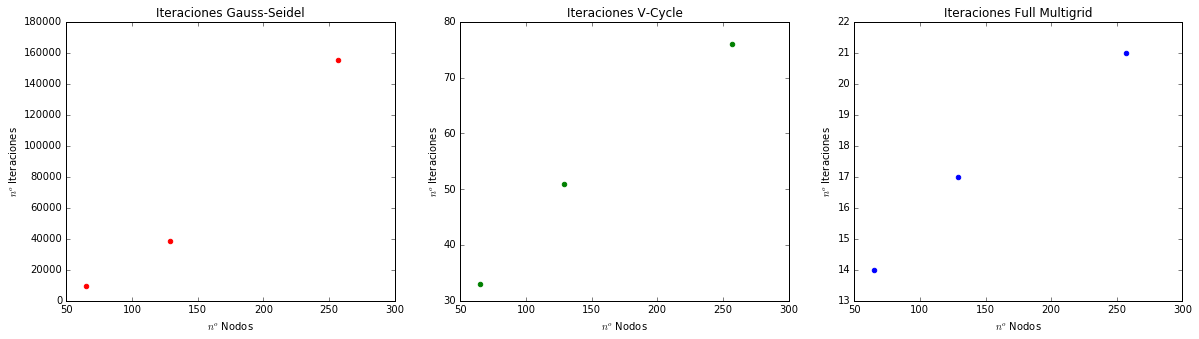
\includegraphics[scale=0.4]{fw_iters.png}
    \caption{Número de iteraciones Full Weighted Restriction}
    \label{fig:fw_iters}
    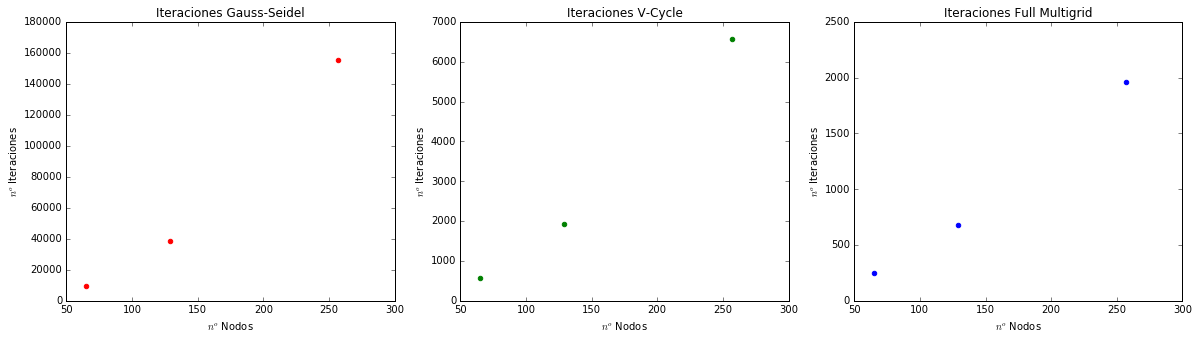
\includegraphics[scale=0.4]{injection_iters.png}
    \caption{Número de iteraciones Injection Restriction}
    \label{fig:iters}
\end{figure}


Pero realizar la comparacion de ciclos de cada algoritmo no es muy representativa, por lo que se calcularon en V-Cycle y FMG la cantidad equivalente de relajaciones Gauss Seidel en la malla fina que se realizaron en total, de lo que resultan las figuras \ref{fig:fw_complex} y \ref{fig:complex}. De estos resultados se aprecia que Gauss Seidel sigue teniendo una gran cantidad de ciclos en comparación a los otros algoritmos, siendo FMG el con menor cantidad de iteraciones equivalentes.

\begin{figure}[H]
    \centering
    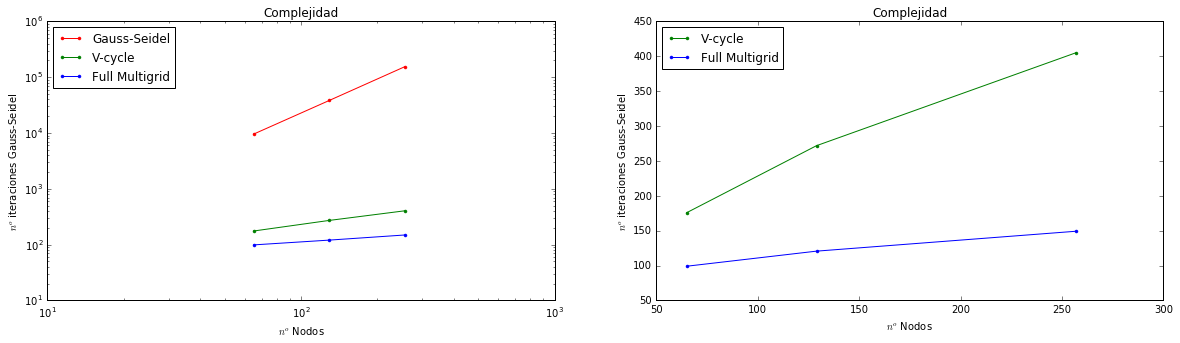
\includegraphics[scale=0.4]{fw_complex.png}
    \caption{Número de iteraciones equivalentes Full Weighted Restriction}
    \label{fig:fw_complex}
    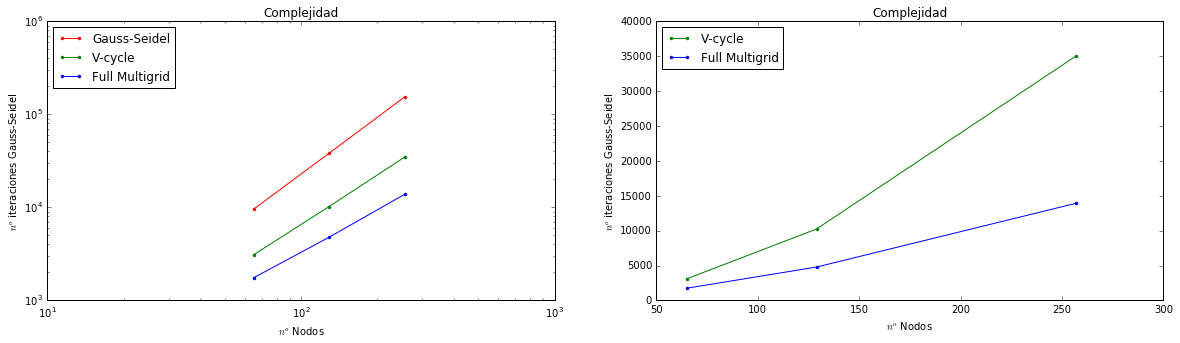
\includegraphics[scale=0.4]{injection_complex.png}
    \caption{Número de iteraciones equivalentes Injection Restriction}
    \label{fig:complex}
\end{figure}


Si dejamos de lado las iteraciones y nos centramos en el tiempo en escala Log-Log (Figuras \ref{fig:fw_t} y \ref{fig:t}). En este caso si podemos observar el comportamiento cuadrático de Gauss Seidel en comparación al lineal de V-Cycle y FMG, pero sólo en el caso de Full Weighted, para Injection la cantidad de tiempo se comienza a acercar. Teniendo en cuenta que el comportamiento lineal teórico de estos algoritmos no toma en cuenta el manejo de memoria al momento de cambiar la grilla podemos decir que el resultado práctico se acerca al teórico.
\begin{figure}[H]
    \centering
    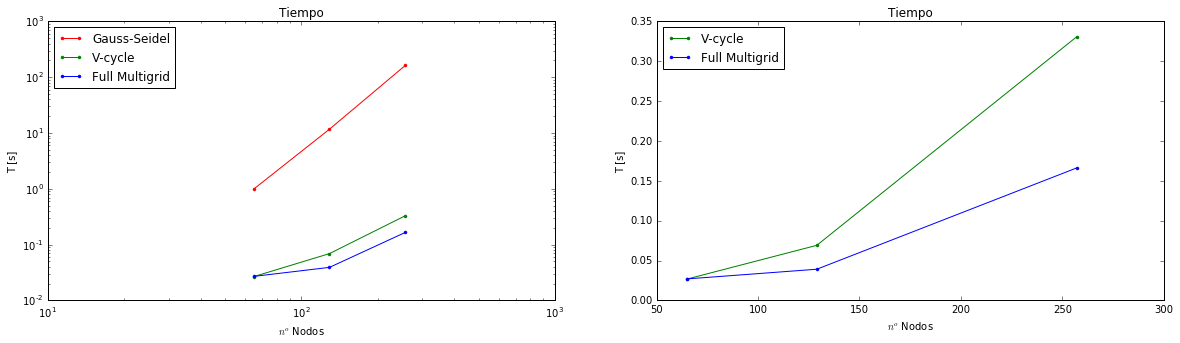
\includegraphics[scale=0.4]{fw_t.png}
    \caption{Tiempo con Full Weighted Restriction}
    \label{fig:fw_t}
    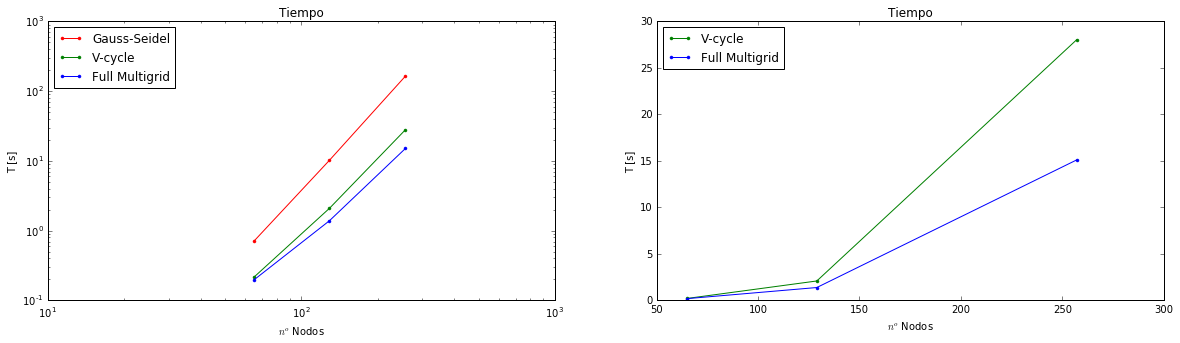
\includegraphics[scale=0.4]{injection_t.png}
    \caption{Tiempo con Injection Restriction}
    \label{fig:t}
\end{figure}


Como se obtuvieron buenos resultados para V-Cycle y FMG se procedió a analizar que tan buena era la solución obtenida, como se observa en las figuras \ref{fig:fw_e} y \ref{fig:e}, en el caso de Gauss Seidel y V-Cycle se encontraron soluciones comparables con un bajo error, el problema se encuentra en el FMG que se estanca en soluciones de no tan buena calidad, esto puede ser debido a que el FMG implementado no resuelve el mismo problema en todas las mallas, por lo que encuentra una solución distinta y para estos casos peor.

\begin{figure}[H]
    \centering
    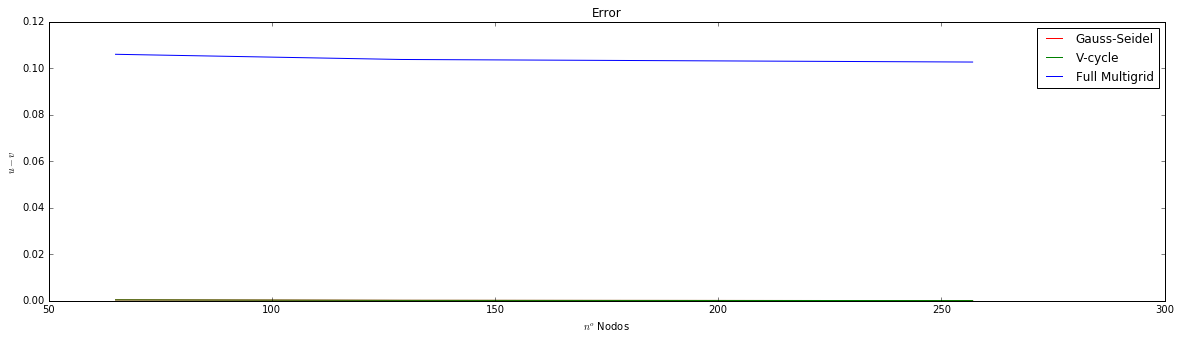
\includegraphics[scale=0.3]{fw_e.png}
    \caption{Error $e=|u-v|$ con Full Weighted Restriction}
    \label{fig:fw_e}
    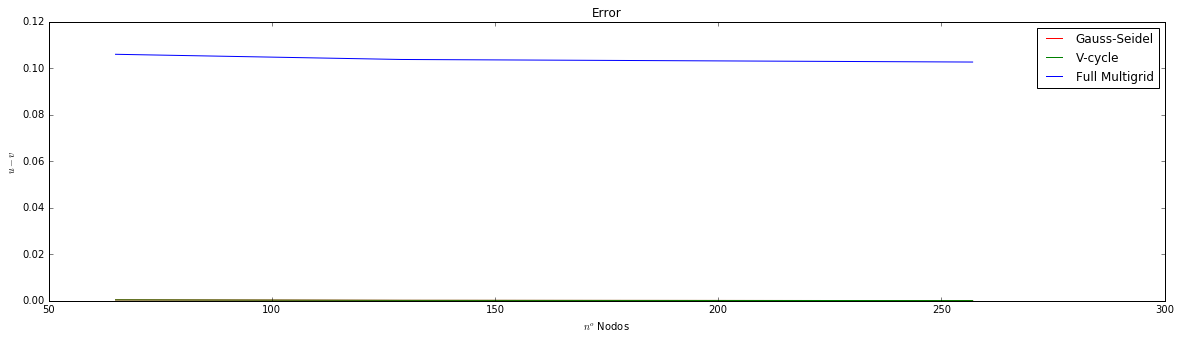
\includegraphics[scale=0.3]{injection_e.png}
    \caption{Error $e=|u-v|$ con Injection Restriction}
    \label{fig:e}
\end{figure}


Si observamos el residual de cada caso vemos que para Gauss Seidel (Figura \ref{fig:gs_e}) y V-Cycle (Figura \ref{fig:v_e}) la mayor cantidad de error se encuentra en la zona central de la solución en cambio para FMG (Figura \ref{fig:fmg_e}) está concentrado en un extremo de la solución.

\begin{figure}[H]
    \centering
    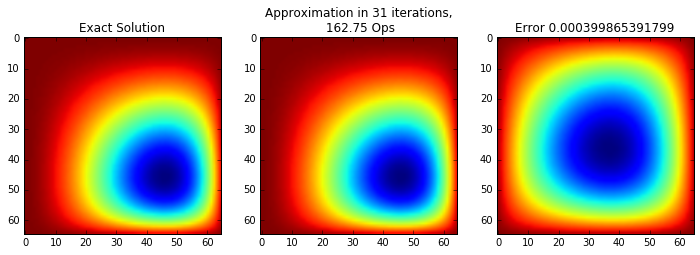
\includegraphics[scale=0.4]{gs_e.png}
    \caption{Error Gauss Seidel }
    \label{fig:gs_e}
    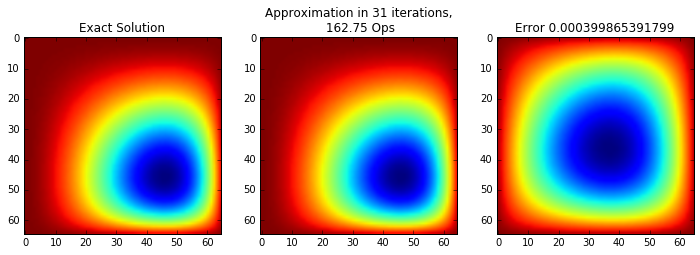
\includegraphics[scale=0.4]{v_e.png}
    \caption{Error V-Cycle }
    \label{fig:v_e}
    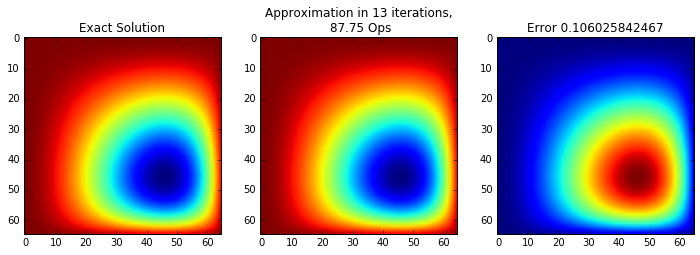
\includegraphics[scale=0.4]{fmg_e.png}
    \caption{Error Full Multigrid }
    \label{fig:fmg_e}
\end{figure}

\subsection{Experimento 2}
En este experimento se buscaba ver cómo afectan los parámetros $\nu_0, \nu_1,\nu_2$ a los distintos algoritmos, para esto se utilizaron los 3 algoritmos variando los parámetros. 

Como se ve en la figura \ref{fig:exp2}, para V-Cycle independiente del parámetro $\nu_1$ se obtuvo un buen resultado, pero cuando $\nu_2$ es 5 se tiene que el error es mayor, como se observó en el experimento 1 la implementación de FMG realizada no es muy buena por lo tanto no se obtuvieron resultados concluyentes variando $\nu_0$

\begin{figure}[H]
\begin{subfigure}{\textwidth}
  \centering
  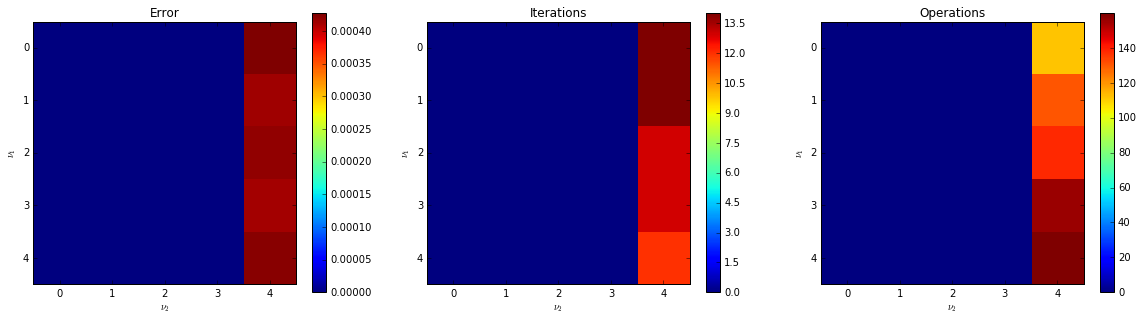
\includegraphics[scale=0.4]{e2_vcycle.png}
  \caption{V-Cycle}
\end{subfigure}
\begin{subfigure}{\textwidth}
  \centering
  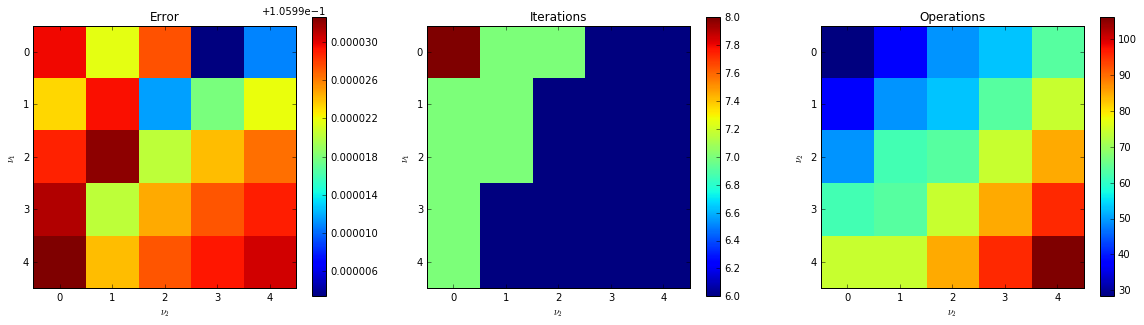
\includegraphics[scale=0.4]{fmg_v0_1.png}
  \caption{FMG $\nu_0=1$ }
\end{subfigure}
\begin{subfigure}{\textwidth}
  \centering
  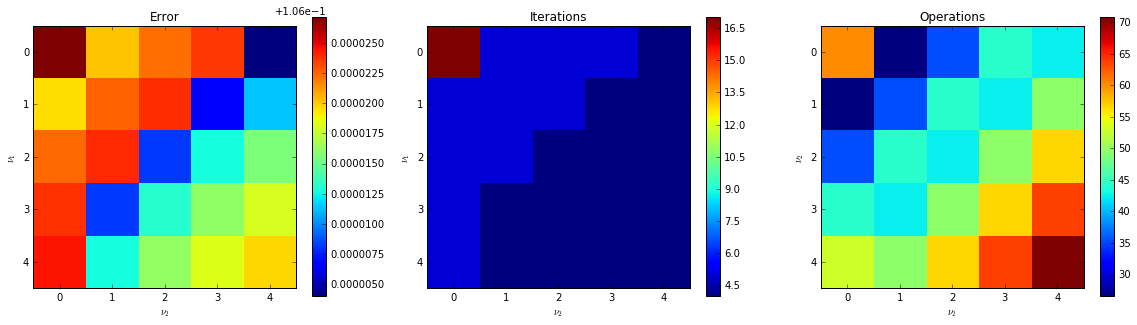
\includegraphics[scale=0.4]{fmg_v0_2.png}
  \caption{FMG $\nu_0=2$ }
\end{subfigure}
\begin{subfigure}{\textwidth}
  \centering
  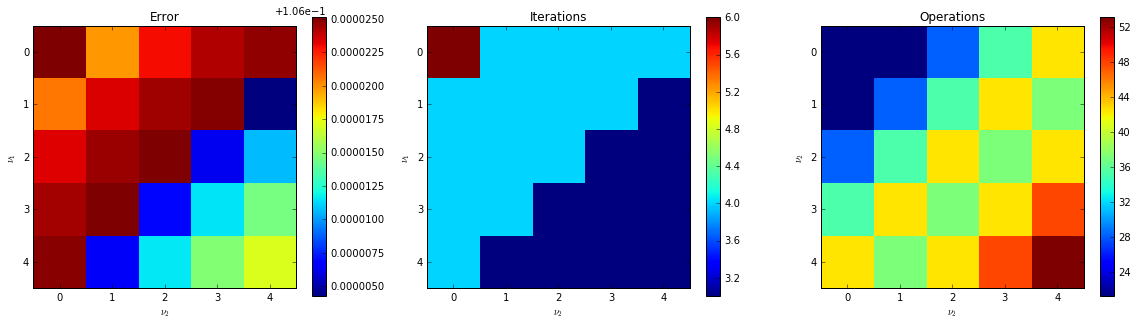
\includegraphics[scale=0.4]{fmg_v0_3.png}
  \caption{FMG $\nu_0=3$ }
\end{subfigure}

    \caption{Experimento 2 variando $\nu_0,\nu_1,\nu_2$}
    \label{fig:exp2}
\end{figure}

\subsection{Conclusiones Generales}

La utilización de algoritmos iterativos para resolver sistemas de ecuaciones lineales en especial Ecuaciones Diferenciales Parciales resulta útil ya que necesitan menor tiempo para poder obtener soluciones en comparación de algoritmos completos como descomposiciones PALU, Cholesky u otro. Puede ser que el error de este tipo de métodos sea mayor pero dependiendo de la aplicación esto puede no ser tan importante, ya que se necesitan buenas aproximaciónes más que resultados exactos.

Por su parte los algoritmos de Multi-Malla como V-Cycle o Full Multigrid ofrecen una convergencia mucho más rápida llegando a tener complejidad lineal al estar bien implementados. En el caso del algoritmo FMG implementado se observó que a pesar de tener una convergencia más rápida encuentra soluciones peores que las de V-Cycle o Gauss Seidel por lo que no es una buena implementación. 

\bibliographystyle{plain}
\bibliography{Referencias}

\end{document} 


